\documentclass{sigchi}

% Remove or comment out these two lines for final version
% \toappearbox{\Large Submitted to CHI'13. \\Do not cite, do not circulate.}
\pagenumbering{arabic}% Arabic page numbers for submission.

% Use \toappear{...} to override the default ACM copyright statement (e.g. for preprints).

% Load basic packages
\usepackage{balance}  % to better equalize the last page
\usepackage{graphics} % for EPS, load graphicx instead
\usepackage{times}    % comment if you want LaTeX's default font
\usepackage{url}      % llt: nicely formatted URLs
\usepackage{cite}      % llt: nicely formatted URLs

% llt: Define a global style for URLs, rather that the default one
\makeatletter
\def\url@leostyle{%
  \@ifundefined{selectfont}{\def\UrlFont{\sf}}{\def\UrlFont{\small\bf\ttfamily}}}
\makeatother
\urlstyle{leo}


% To make various LaTeX processors do the right thing with page size.
\def\pprw{8.5in}
\def\pprh{11in}
\special{papersize=\pprw,\pprh}
\setlength{\paperwidth}{\pprw}
\setlength{\paperheight}{\pprh}
\setlength{\pdfpagewidth}{\pprw}
\setlength{\pdfpageheight}{\pprh}

% Make sure hyperref comes last of your loaded packages,
% to give it a fighting chance of not being over-written,
% since its job is to redefine many LaTeX commands.
\usepackage[pdftex]{hyperref}
\hypersetup{
pdftitle={SIGCHI Conference Proceedings Format},
pdfauthor={LaTeX},
pdfkeywords={SIGCHI, proceedings, archival format},
bookmarksnumbered,
pdfstartview={FitH},
colorlinks,
citecolor=black,
filecolor=black,
linkcolor=black,
urlcolor=black,
breaklinks=true,
}

% create a shortcut to typeset table headings
\newcommand\tabhead[1]{\small\textbf{#1}}


% End of preamble. Here it comes the document.
\begin{document}

\title{Peereviz: Visualizing Peer Reviews}

% Note that submissions are blind, so author information should be omitted

\author{
  \alignauthor Kanit Wongsuphasawat, Chih-Chiang Wei, Thiraphat Charoensripongsa\\
    \affaddr{Stanford University}\\
    \email{\{kanitw, ccwei, tchar\}@stanford.edu}\\
}


% Teaser figure can go here
%\teaser{
%  \centering
%  \includegraphics{Figure1}
%  \caption{Teaser Image}
%  \label{fig:teaser}
%}

\maketitle

\begin{abstract}

% TODO rewrite this at the end!

Peer reviews is a one possible in scaling assessment of open-ended assignment in
massive online open courses (MOOCs).  However, the amount of data from peer
review process is huge and it becomes difficult to explore and understand.  In
this paper, we present Peereviz, an exploration tool for large-scale peer review
that helps course instructors to understand and gain insights from the peer
review activities, the engagement of students, and the quality of the reviews.
Peereviz utilized existing text visualization techniques as well as  Multiple
Coordinated Views and enable the quick navigation through original feedbacks.
\end{abstract}

\keywords{
	peer review; group collaboration; visualization; MOOC; exploration;
  text visualization
}
	% \\\textcolor{red}{Mandatory section to be included in your final version.}
% }

% \category{H.5.m.}{Information Interfaces and Presentation (e.g. HCI)}{Miscellaneous
% \\
% \textcolor{red}{See: \url{http://www.acm.org/about/class/1998/}
% for more information and the full list of ACM classifiers and descriptors.
% Mandatory section: On the submission page
% only the classifiers' letter-number combination will need to be entered.}
% }

% \terms{
% 	Human Factors; Design; Measurement.
% 	If you choose more than one ACM General Term,
% 	separate the terms with a semi-colon.
% \\
% \textcolor{red}{If you choose more than one ACM General Term,
% separate the terms with a semi-colon. See list of ACM terms at:
% \url{http://www.sheridanprinting.com/sigchi/generalterms.htm}.
% Optional section to be included in your final version.}
% }


\section{Introduction}
Massive open online courses(MOOCs) including Khan Academy, Udacity, Coursera and
Venture Lab are increasing in numbers \cite{nytimes}. One emerging challenge is
how to scale assessment to these high student-teacher ratio environments.
For assignment that have clear representative answer
such as multiple choices questions,
automated grading system can be employed.
While human graders are still needed for the assessment of open-ended assignments.

Using peer review system \cite{cpr}, i.e. having each student grade each other,
to assess students’ work is another possible solution.
However, in the massive online courses, the number of reviews done in each class
is large and it is overly difficult
and time-consuming for instructors to get a comprehensive understanding
of the review of each task.

To address this problem, we developed Peereviz, a peer review exploration tool
on top of Venture Lab platform. It aims for helping instructors to understand
the massive amount of peer review results. The design goal of the tool is to
create a visualization tool that helps course instructors in three ways:

\begin{enumerate}
\item get the overall understanding of peer review activities;
\item be able to dive into specific part of the review results;
\item quick browse and select higher quality reviews to read.
\end{enumerate}

As a data explorer, it follows ``overview first, zoom and filter, then details-
on-demand mantra'' \cite{card1999readings}.


The paper organization is as follows.
We first summarize previous work in peer review system and visualization.
We then describe the peer review data we used.
Next, we present our design and visualization techniques,
followed by the evaluation and feedbacks from users.
Finally, we suggest the possible directions for future work
and then summarize our work.



\begin{figure}[!t]
\centering
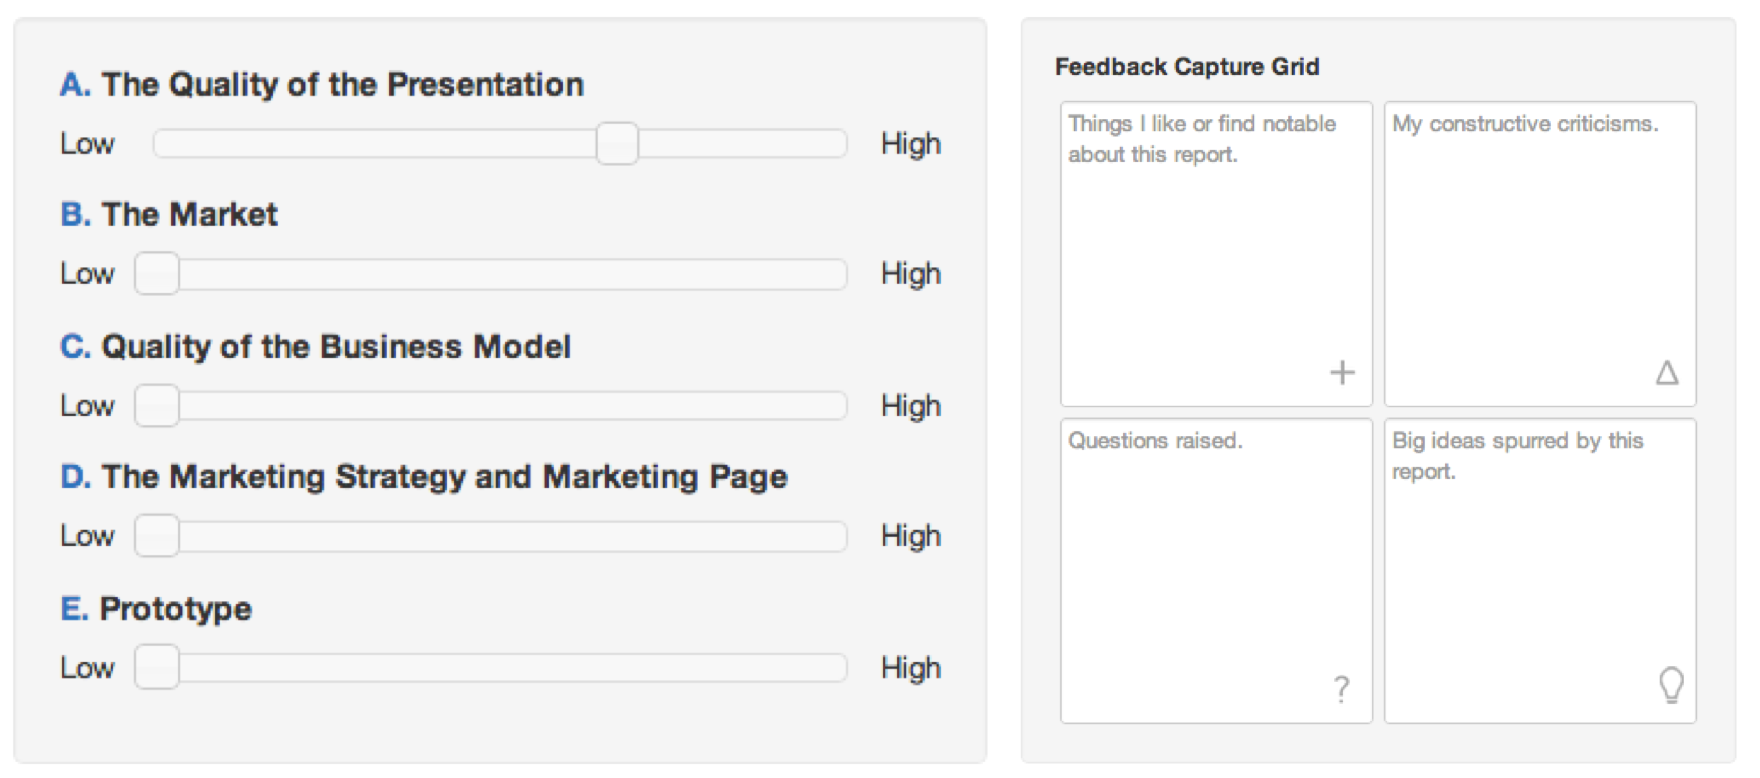
\includegraphics[width=\columnwidth]{images/review-form}
\caption{the actual evaluation form on the Venture lab platform.
The top part shows the quantitative feedbacks which are score ranging
from Low (1) to High (10) while the bottom part shows the feedback capture grid
which a form where the reviewers give their opinions
on four different aspect: notable, constructive, questions, and ideas.}
\label{fig:review-form}
\end{figure}


\section{Related Work}

A number of studies has confirmed the usefulness of the peer review system
to the students in various domains including programming, writing and design classes
\cite{MyPeerReview,WebBasedPeerReview,de2009assessment}.

However, to the best of our knowledge, work that combines visualization
techniques to help instructors understand peer review data is still limited.
The only work we discovered is  an interactive tool for peer-review
exploration proposed by Xiong et al. \cite{xiong} They primarily work on the
improvement of semantic information to help instructor discover interesting
patterns and compare different groups of student in the writing class on SWoRD
system \cite{Cho2007}. In contrast to the prior work, we mainly focuses on the
visualization and interaction design for exploring multi-dimensional peer
review data in the recently emerging large-scale online courses.


\begin{figure*}[ht]
\centering
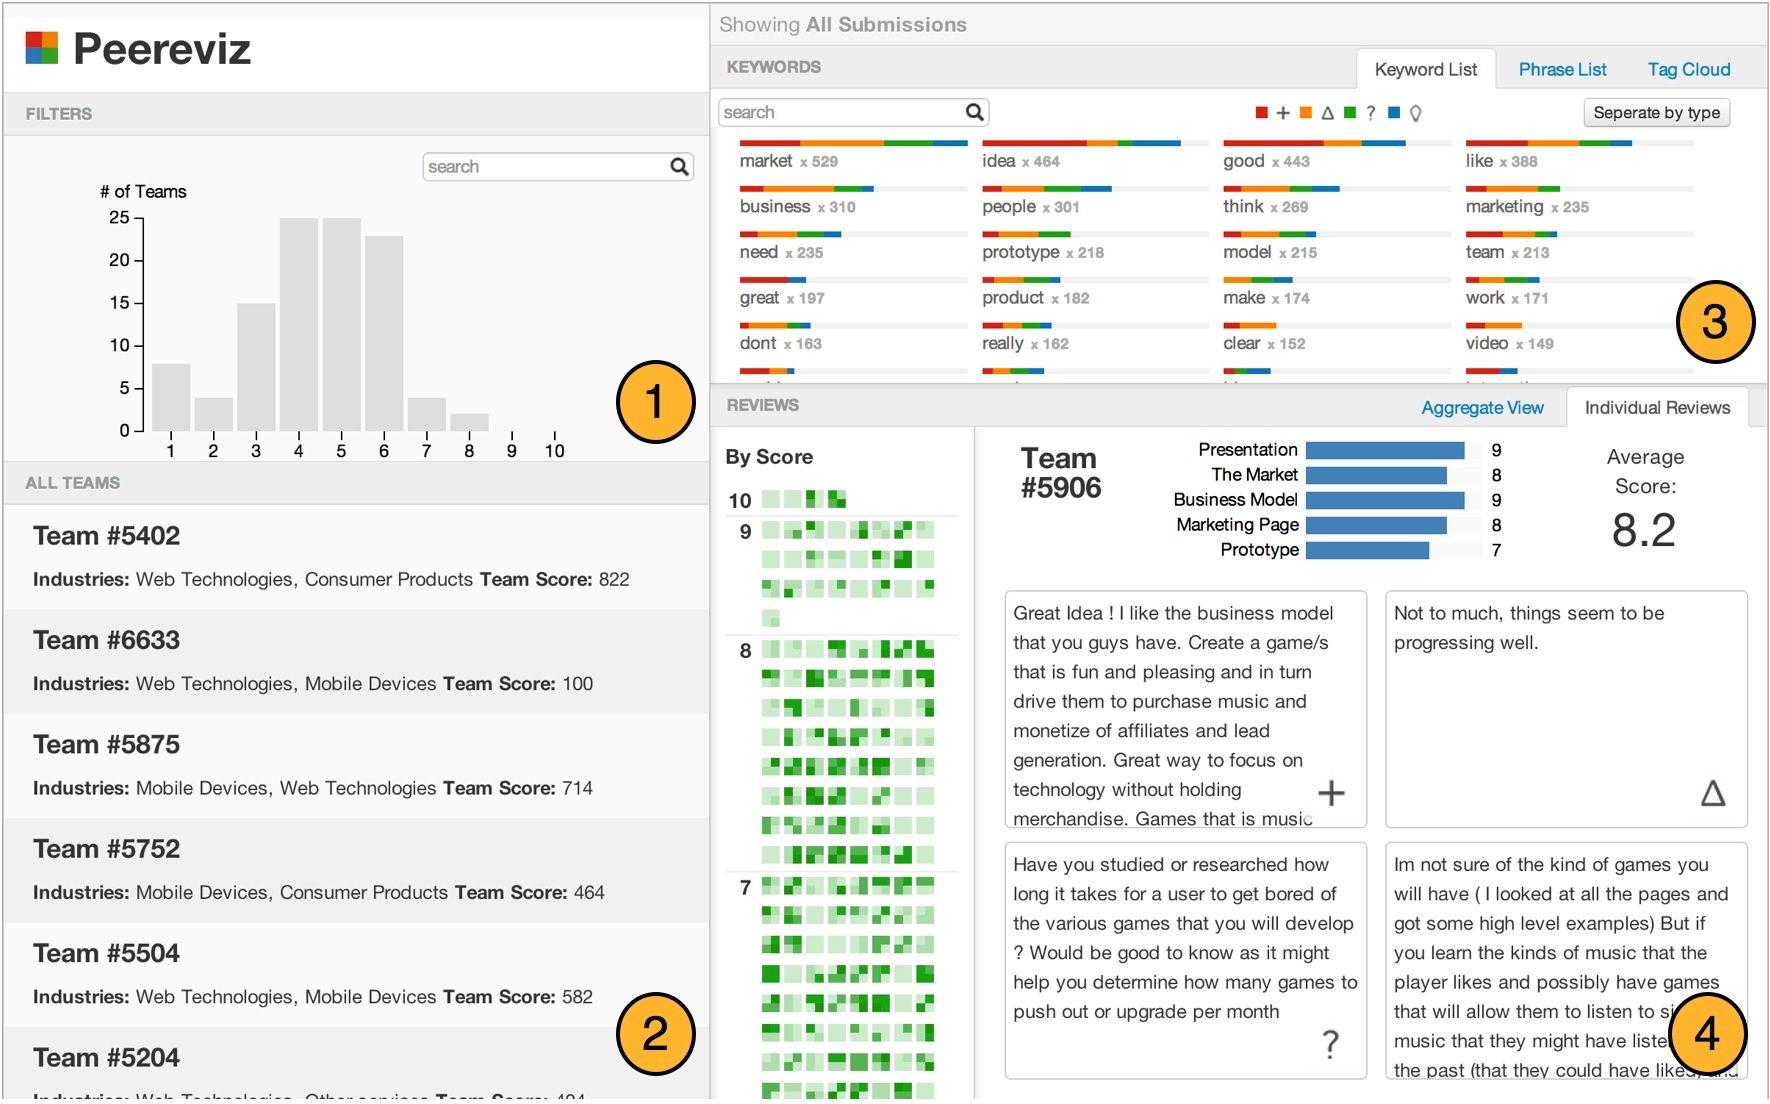
\includegraphics[width=2.0\columnwidth]{images/overview-annotated}
\caption{The layout for Peereviz is divided into two parts:
the team browser (1,2) and the review browser (3,4).
(1) shows the overall score distribution,
(2) team description list,
(3) keyword list, and
(4) Aggregate and individual reviews.}
\label{fig:overview-annotated}
\end{figure*}

\section{Data Set Description}
We use a sample data set from a final project peer review result in the Spring
2012 Entrepreneurship class on the Venture Lab platform. A total of 1,206 peer
reviews are collected, which consists of 116 teams being reviewed and 212
individual reviewers. For privacy reasons, the team names are anonymized and we
presented team description as much as needed. The actual peer review form has
two parts, including multiple quantitative score ranging from Low (1) to
High (10) for different aspects of the final project and qualitative text
feedback, which utilizes a feedback capture grid \cite{dbootcamp} where
reviewers could express their opinions in four dimensions --- what they
like (\emph{notable}), constructive criticisms (\emph{constructive}), questions
they have about the work (\emph{questions}), and any additional ideas for the
project (\emph{ideas}).



\section{Visualization Design}
We use multiple coordinated views techniques to
show data in different representations which enable users to interact, explore
and understand intricate data \cite{roberts2007state}. Furthermore, we also
use text visualization techniques, including word count list and tag cloud,
which are often used to visualize and understand various large text data
\cite{kuo2007tag, wordcountwww}.

\subsection{Layout}
As one of our design goals is to provide fast navigation,
we put all views in one page so the user do not need to scroll or find hidden
menu to achieve their intended tasks. The layout, as shown in Figure
\ref{fig:overview-annotated}, consists of two parts,
the team browser and the review
browser.  The first is the team browser on the left side, which contains a
team list and a bar chart that visualizes overall score distribution for all
team projects. The second is the review browser on the right side which
consists of two sub-parts: the keyword visualization for browsing keyword on
the upper part and review display view on the bottom part.

\begin{figure}[]
\centering
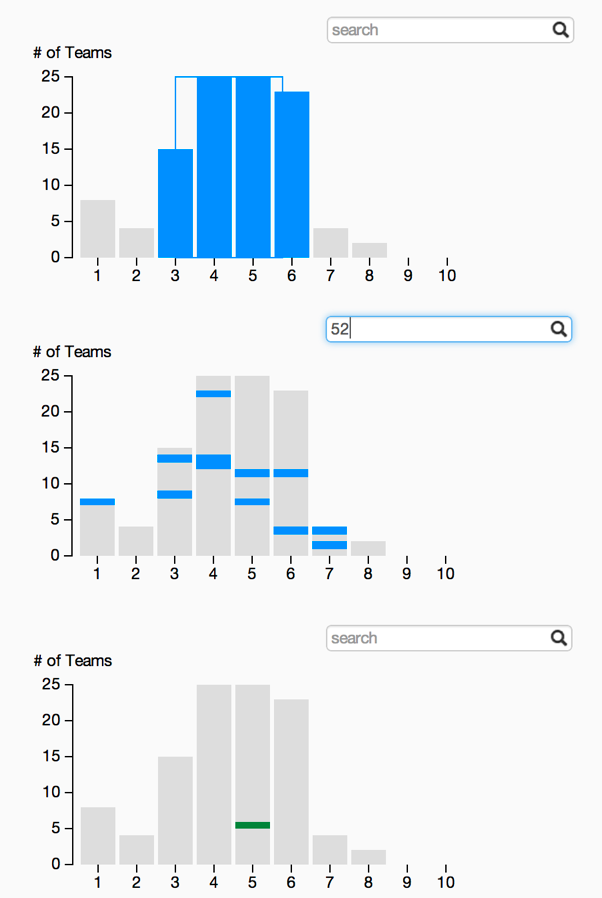
\includegraphics[width=\columnwidth]{images/3charts}
\caption{Different selection modes in the team browser.
The top one shows brushing mode, which can be used to select teams within a range of scores.
The middle one shows search mode, which user can use text by-description search.
The bottom one show one team selection, by click on a block on the stacked bar chart.}
\label{fig:keyword-lists}
\end{figure}


\begin{figure}[]
\centering
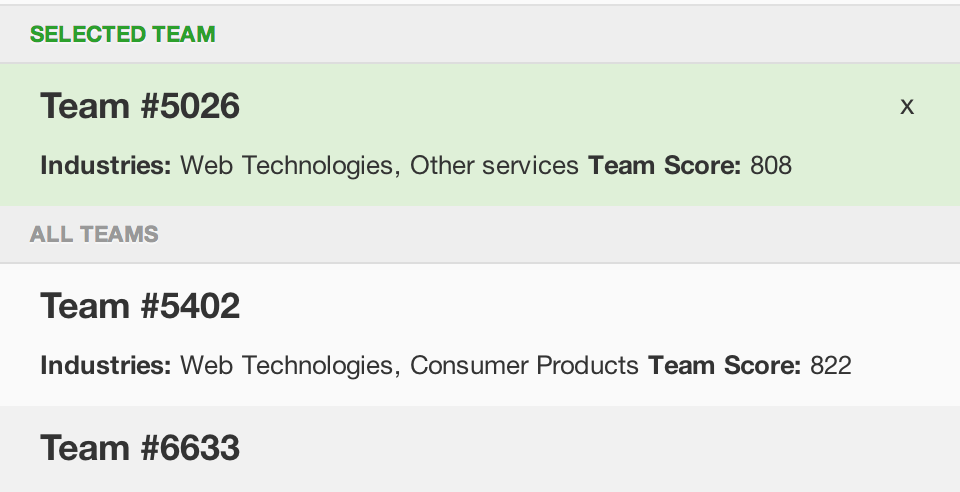
\includegraphics[width=.8\columnwidth]{images/selected-team}
\vspace{2.00mm}
\caption{If the user select a team, either from the stacked bar chart or from the list,
a selected team page will appear to help user recognize that a team has been selected.}
\label{fig:selected-team}

\end{figure}

\subsection{Team Browser}
The team browser serves as the main part of the overview
where we can select one or multiple teams using different ways of filtering.

We can select one team by clicking one of the small block on the stacked bar
chart or select multiple teams at the same time by brushing over the bar chart.
After the selection, the team descriptions will be listed below as noted by (2)
in Figure \ref{fig:overview-annotated}. The information provided in the review
browser will be updated accordingly with the data of the selected team(s). In
addition, it provides a search tool to select teams by their descriptions as
well.



\subsection{Review Browser}
The review browser shows data for the selected team(s) in the team browser. If
the user has not selected any team in the team browser, the review browser
provides overview by showing aggregated data of all teams.

\subsubsection{Keyword List, Phrase List and Tag Clouds}
Since one major
component of the review is qualitative text feedbacks, we extracted keywords
from text feedbacks based on their term frequency in bag-of- words model \cite
{bag-of-words} to provide an overview of what students wrote the most in their
reviews. There are three representations: keyword list, phrase list and tag
cloud. In any of the three modes, users can click any word to see the actual
occurrence of the word to further understand the context of the word.


\begin{figure*}[]
\centering
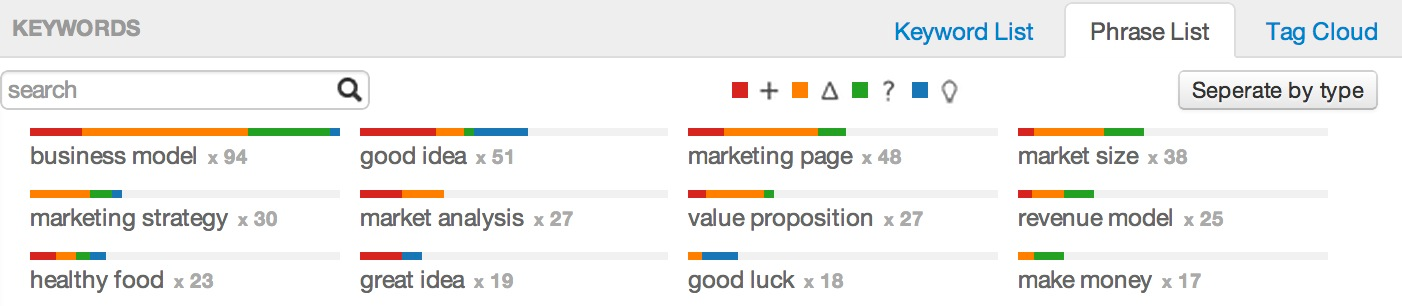
\includegraphics[width=1.4\columnwidth]{images/phrase-list}
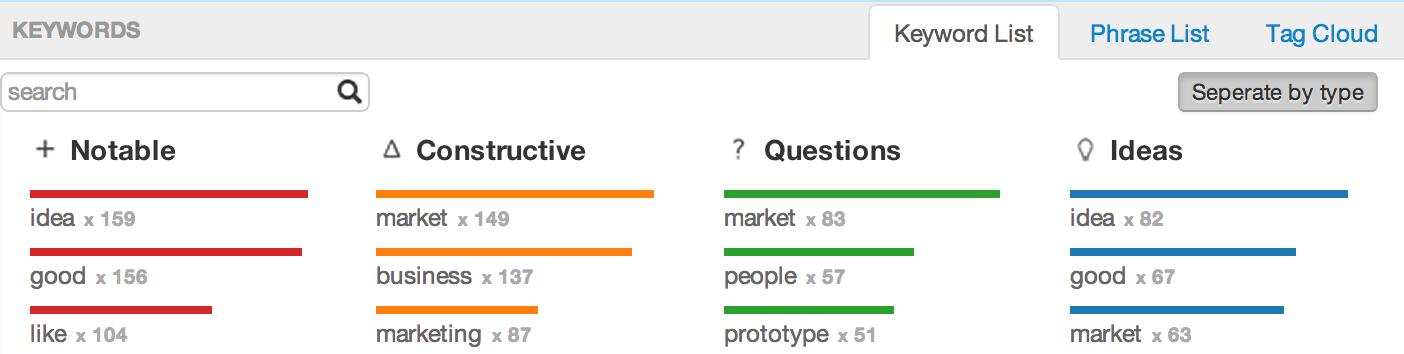
\includegraphics[width=1.4\columnwidth]{images/keyword-list}
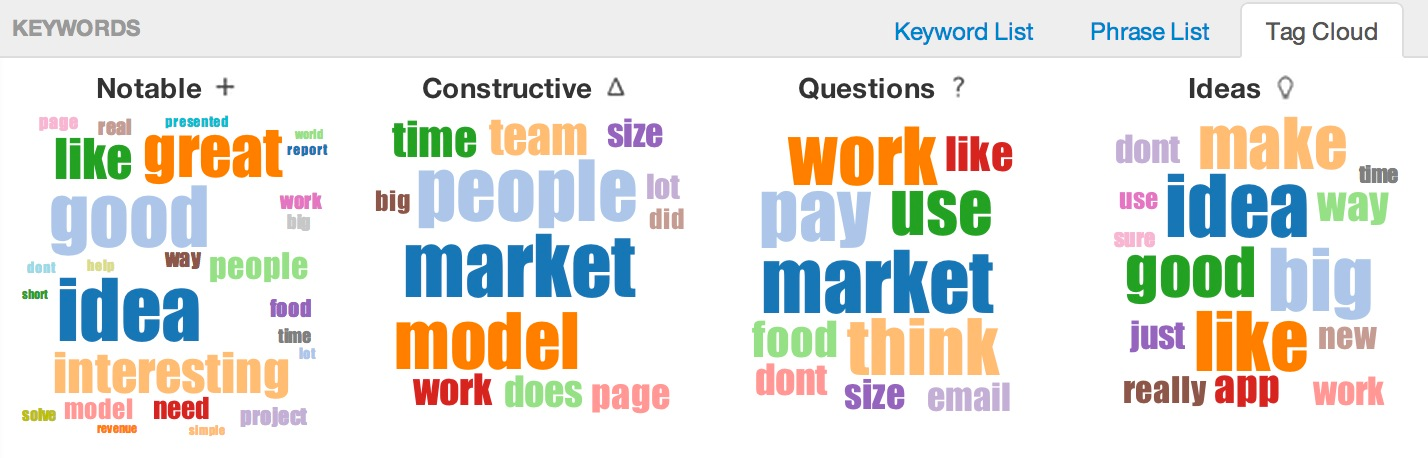
\includegraphics[width=1.4\columnwidth]{images/clouds}
\caption{Three views of the keyword browser:
(top) the phrase list in integrated mode,
(middle) the keyword list in group-by-type mode,
(bottom) the tag clouds grouped by type.}
\label{fig:keyword-lists}
\end{figure*}

The keyword list and phrase list are sorted lists by unigram and bigram term
frequency respectively.  Each word in the frequently list shows a bar
representing their frequencies in the histogram on top of the word.  There are
two representations for the frequency lists: The first view shows keywords in
four columns, in which each column represent keywords from different types of
feedback in the original feedback capture grid. The second view (Upper in
Figure \ref{fig:keyword-lists}) shows the total frequency of the words
aggregated from all the feedback types.  In this view, we use color to
encoding the proportion of the keyword from each type.

Both frequency list views show the most frequent words on the top.  User can
also use the search box to search for unigram or bigram they are interested in.
Meanwhile, the tag clouds view show four tag clouds of keywords group by each
type in the feedback capture grid.  Our tag clouds display all words
horizontally for ease of reading.


\begin{figure*}[]
\centering
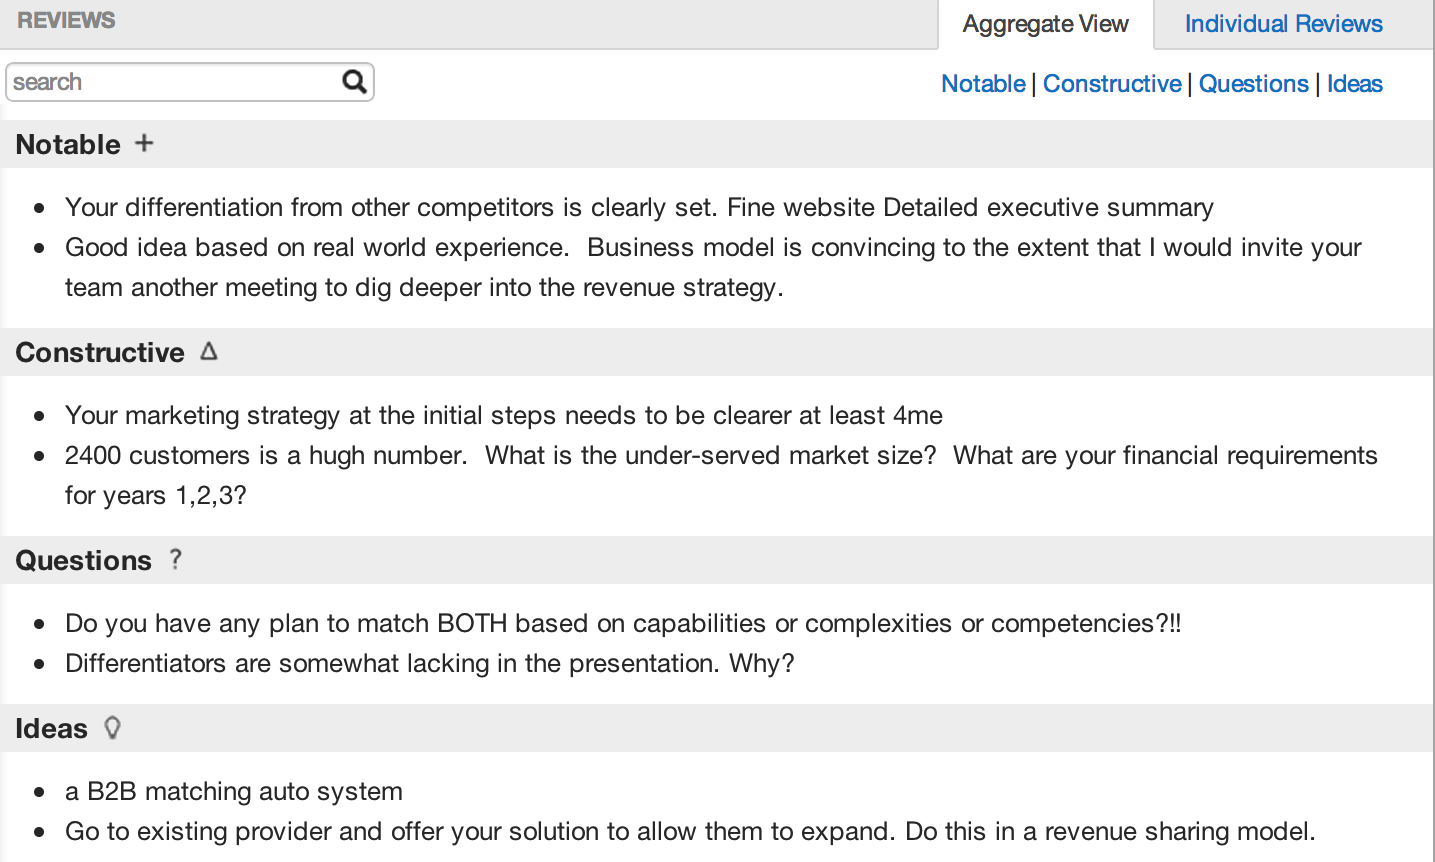
\includegraphics[width=1.4\columnwidth]{images/aggregate-view}
\caption{Aggregate View.}
\label{fig:aggregate-view}
\end{figure*}

\subsubsection{Aggregate View and Individual Review View}


\begin{figure*}[]
\centering
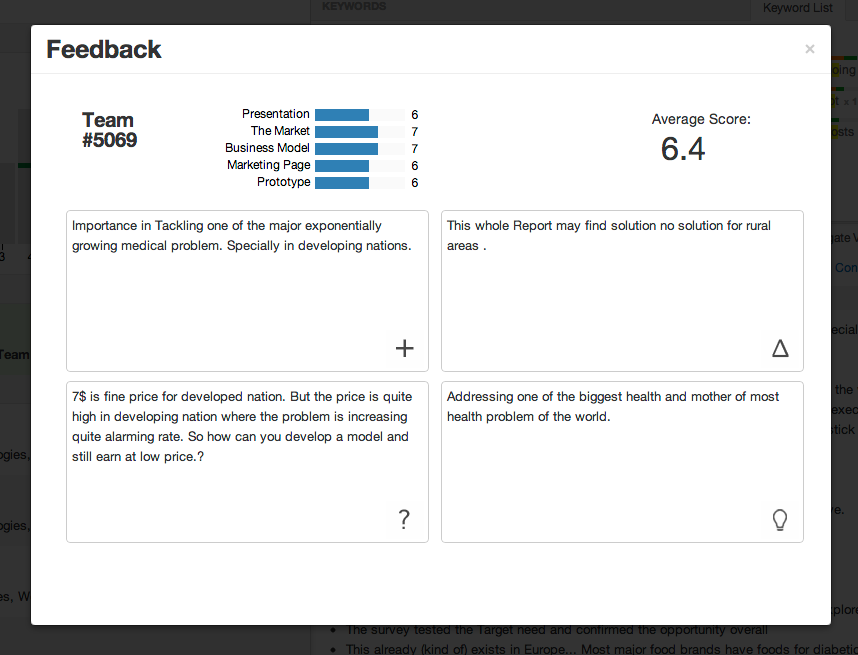
\includegraphics[width=1.4\columnwidth]{images/modal}
\caption{A Modal dialog showing original review rata after
 a user click on a review data in the Aggregate View.}
\label{fig:modal}
\end{figure*}


\begin{figure*}[]
\centering
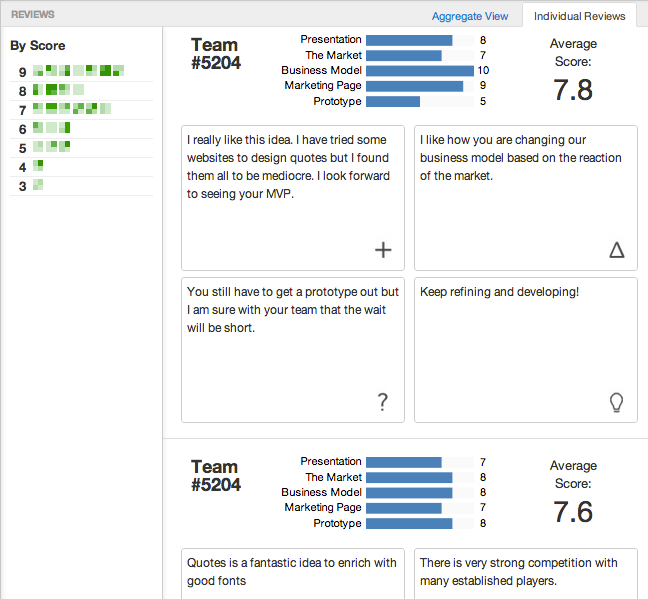
\includegraphics[width=1.4\columnwidth]{images/ind-review-view}
\caption{Individual Review View.}
\label{fig:ind-view}
\end{figure*}


In aggregate view, the text feedbacks for the selected teams are shown
separately categorized by their types from feedback capture grid. This view
provides instructors a quick way to read through a number of reviews for each
feedback type at a time. As usual, it provides a search tool so users can
search through the text feedbacks.

Individual reviews view is used to browse through the original reviews. It
consists of two main parts as shown in Figure \ref{fig:ind-view}. First part
on the left is a list of small multiples, and each small grid corresponds to
single original review. We use color encoding in the small grid to represent
the length of the review text: the longer the review text, the more intense
the color is; so that the instructors can quickly read and select longer
reviews which are potentially more valuable to read. The user can click small
multiples to navigate through the original review list. Each original review
item in the list contains the original scores distribution for the rubrics,
the average score, and the feedback capture grid as in the original form.





\section{Implementation Notes} Peereviz was written in HTML, CSS and
Javascript using the d3.js visualization toolkit \cite{d3} and a combination
of javascript libraries including jQuery, Underscore.js, Backbone.js
\cite{jquery,underscore,backbone}.  The d3’s design that utilizes existing web
standards including SVG and HTML has greatly facilitated our implementation.

One advantage of developing Peereviz in Javascript and HTML is that it could
be easily integrated to any other online platforms since no other server-side
setup is needed as opposed to developing the entire system using Ruby on rails
and implementing different controllers to handle different pages.

As for the data processing, we performed SQL queries to get all the data we
need and imported it directly at once. It also provides the plug-and-play
convenience since users don't have to have a database or remote server to
provide the data. But it might not be a good idea when the data size becomes
too large. Directly loaded it from database or split the data into separate
files and load them as needed might be another alternative but it might slow
it down due to the data I/O as well.

\section{Discussion and Future Work}

This visualization has provided a way for course instructors to
quickly browse the peer review data and get senses of the ongoing peer review
activities.

We have presented Peereviz to Venture Lab administrator and let her play with it for
30 minutes.  She has expressed her positive feedback of this tool and mentioned
that she hope to use this to find out what are qualities of team that get good grades
and what has gone  wrong for teams with a low grade.  She believes that the pattern
discovered from this tool can provide helpful feedback for both future offering
of the courses and the design of the platform.
We plan to further evaluate this tool from real instructor usage in online classes
after we integrate it into the Venture Lab platform.

In terms of improvement, one area that we can improve is the text visualization techniques.
Our current
work has only ranked it by the word frequency, while we could easily replace the
underlying calculation for ranking the words. For example, we could instead use
TF-IDF model \cite{manning2008} or other score calculations to find more
expressive words.

We have also learned that visualization of the review also largely depends on
the peer review form.  Pre-structured form facilitates greatly in making the
visualization.  Our visualization benefits from the feedback capture employed in
the platform.  Thus, we suggest that providing scaffolding structure in the peer
evaluation form does not only improve the review quality but also help the
teaching teams to better understand the result as well.

Finally, another possible improvement is to enhance system’s ability to compare
different group of students by demographic such as GPA, academic major, or
nationality.


% this can be 'Usage Observation' (http://www.danah.org/papers/InfoViz2005.pdf)

\section{Conclusion}

In this paper, we described the visualization design of Peereviz, a system for
exploring the peer review data in massive online open courses.   We employed
techniques from text visualization, simple language modeling and multiple
coordinated views to help course instructors explore the result of assessments
and learning outcomes as well as the insights from the overall peer review
activities. In the near future, we are going to integrate this additional
visualization feature to the Venture Lab platform.

\section{Acknowledgments}
The authors of this paper would like to thank Farnaz Ronaghi and Venture Lab
team for providing data and suggestions.
Jeff Heer and CS448b (Data Visualization) course teaching team's comment
and suggestions are also appreciated.

% Balancing columns in a ref list is a bit of a pain because you
% either use a hack like flushend or balance, or manually insert
% a column break.  http://www.tex.ac.uk/cgi-bin/texfaq2html?label=balance
% multicols doesn't work because we're already in two-column mode,
% and flushend isn't awesome, so I choose balance.  See this
% for more info: http://cs.brown.edu/system/software/latex/doc/balance.pdf
%
% Note that in a perfect world balance wants to be in the first
% column of the last page.
%
% If balance doesn't work for you, you can remove that and
% hard-code a column break into the bbl file right before you
% submit:
%
% http://stackoverflow.com/questions/2149854/how-to-manually-equalize-columns-
% in-an-ieee-paper-if-using-bibtex
%
% Or, just remove \balance and give up on balancing the last page.
%
%\balance

% If you want to use smaller typesetting for the reference list,
% uncomment the following line:
% \small
\bibliographystyle{acm-sigchi}
\bibliography{peerevis}

\end{document}
